\chapter{Polímeros}\label{ch:g12:polymers}

Un forro polar puede hilarse a partir de botellas de bebida fundidas; una
cuerda de escalada está hecha de nailon; esta página es celulosa,
fabricada por los árboles. Los tres son \omterm{def:g12:polymers:polymer}{polímeros}: \omterm{def:g7:atoms-and-molecules:molecule}{moléculas} de miles de
\omterm{def:g7:atoms-and-molecules:atom}{átomos} de longitud, construidas repitiendo una y otra vez una pequeña
unidad. Sus propiedades ---blandos o rígidos, elásticos o quebradizos,
fusibles o no--- dependen menos de los \omterm{def:g7:atoms-and-molecules:atom}{átomos} que contienen que de la
forma en que se disponen sus largas cadenas.

\begin{recall}
Los \omterm{def:g8:plastics:plastic}{plásticos} están formados por \omterm{def:g7:atoms-and-molecules:molecule}{moléculas} muy largas; los
\omterm{def:g8:plastics:thermoplastic}{termoplásticos} se reblandecen al calentarlos y los \omterm{def:g8:plastics:thermoplastic}{termoestables} no
(\cref{ch:g8:plastics}). Los grupos \omterm{def:g11:functional-groups:alcohol}{alcohol}, ácido, \omterm{def:g11:functional-groups:carboxylic-acid}{éster}, \omterm{def:g11:functional-groups:amine}{amina} y \omterm{def:g11:functional-groups:amine}{amida}
(\cref{ch:g11:functional-groups}). Una adición une dos \omterm{def:g7:atoms-and-molecules:molecule}{moléculas} en una
sola sin perder ningún \omterm{def:g7:atoms-and-molecules:atom}{átomo}
(\cref{ch:g12:curly-arrows}).
\end{recall}

\begin{omfigure}
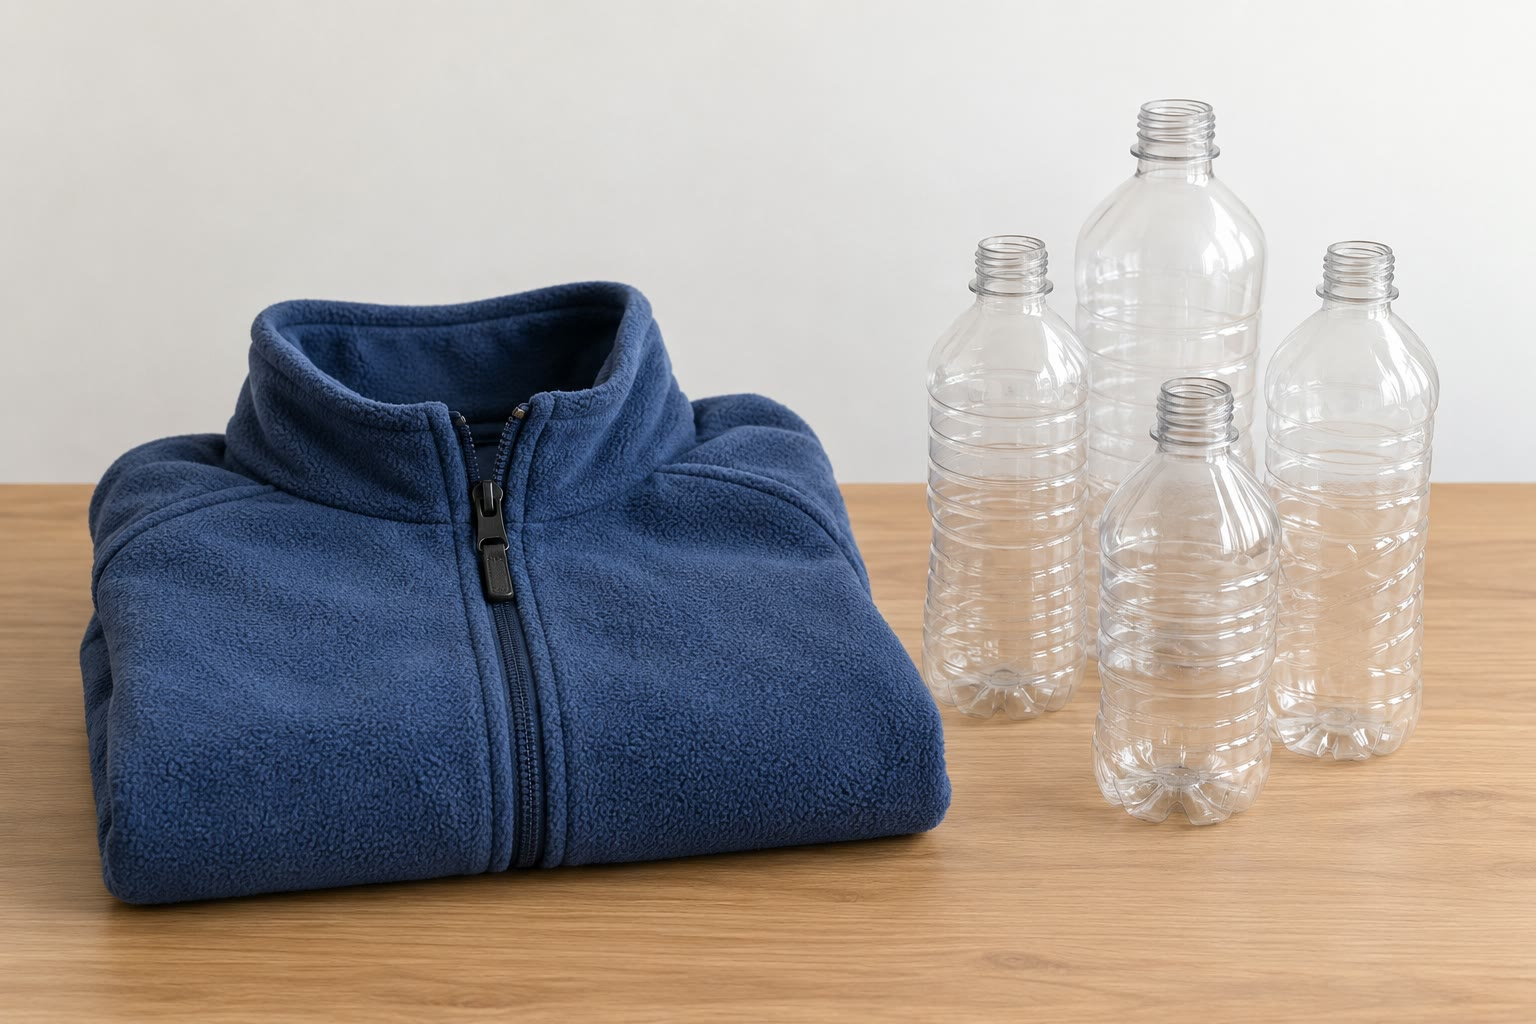
\includegraphics[width=0.45\linewidth]{images/book1/ai/g12-fleece-bottles.jpg}

{\small Botellas de bebida usadas y un forro polar: el mismo \omterm{def:g12:polymers:polymer}{polímero},
con dos formas.}
\end{omfigure}

\section{Monómeros, polímeros, unidades de repetición}

\begin{definition}[Polímero, monómero, polimerización]\label{def:g12:polymers:polymer}
Un \emph{polímero}\index{polimero@polímero} es una sustancia formada por \omterm{def:g7:atoms-and-molecules:molecule}{moléculas}
muy grandes, las macromoléculas, cada una construida a partir de muchas
unidades pequeñas enlazadas una tras otra. Las \omterm{def:g7:atoms-and-molecules:molecule}{moléculas} pequeñas a
partir de las que se fabrica son sus \emph{monómeros}\index{monomero@monómero}; la
reacción que las une es una \emph{polimerización}\index{polimerizacion@polimerización}.
\end{definition}

\begin{definition}[Unidad de repetición, grado de polimerización]\label{def:g12:polymers:repeat-unit}
La \emph{unidad de repetición}\index{unidad de repeticion@unidad de repetición} de un \omterm{def:g12:polymers:polymer}{polímero}
es el grupo de \omterm{def:g7:atoms-and-molecules:atom}{átomos} más pequeño cuya repetición da la cadena; se
escribe entre corchetes con un \omterm{def:g7:atoms-and-molecules:formula}{subíndice} $n$. El número $n$ de unidades
de repetición de una cadena es su \emph{grado de
polimerización}\index{grado de polimerizacion@grado de polimerización}.
\end{definition}

\begin{omfigure}
\[
  n\;\ce{CH2=CH2}
  \quad\longrightarrow\quad
  \chemfig{-[@{op1,.75}]CH_2-CH_2-[@{cl1,0.25}]}
  \polymerdelim[height=6pt, depth=6pt, indice=n]{op1}{cl1}
\]

{\small La \omterm{def:g12:polymers:polymer}{polimerización} del eteno: $n$ \omterm{def:g7:atoms-and-molecules:molecule}{moléculas} de \omterm{def:g12:polymers:polymer}{monómero} dan una
cadena de polietileno, cuya \omterm{def:g12:polymers:repeat-unit}{unidad de repetición} \ce{-CH2-CH2-} se
escribe entre corchetes.}
\end{omfigure}

\begin{proposition}[Masa molar de un polímero]\label{prop:g12:polymers:molar-mass}
Una cadena de \omterm{def:g12:polymers:repeat-unit}{grado de polimerización} $n$ tiene una \omterm{def:g10:the-mole:molar-mass}{masa molar}
\[
  M(\text{polímero}) \approx n \times M(\text{unidad de repetición}) ,
\]
ya que los dos extremos de la cadena son despreciables para $n$ grande.
\end{proposition}

\begin{proof}
La cadena son $n$ \omterm{def:g12:polymers:repeat-unit}{unidades de repetición} más dos grupos terminales de
unos pocos \omterm{def:g7:atoms-and-molecules:atom}{átomos} cada uno; para $n$ del orden de miles, los grupos
terminales pesan menos de una milésima parte del total.
\end{proof}

\begin{example}[Una cadena de polietileno]\label{ex:g12:polymers:pe}
% ledger: aw:C, aw:H
Una cadena de polietileno de \omterm{def:g10:the-mole:molar-mass}{masa molar} \qty{280000}{g/mol} tiene
$n = 280000/28.0 = 10000$ \omterm{def:g12:polymers:repeat-unit}{unidades de repetición}, es decir, veinte mil
\omterm{def:g7:atoms-and-molecules:atom}{átomos} de carbono en fila. En una muestra real, las cadenas no tienen
todas la misma longitud: $n$ es un promedio.
\end{example}

\section{Polímeros de adición}

\begin{definition}[Polímero de adición, polímero de condensación]\label{def:g12:polymers:addition-polymer}
Un \emph{polímero de adición}\index{polimero de adicion@polímero de adición} se forma por
adiciones de \omterm{def:g12:polymers:polymer}{monómeros} que llevan un \omterm{def:g10:lewis-and-shape:multiple-bond}{doble enlace} \ce{C=C}, sin ningún
otro producto: su \omterm{def:g12:polymers:repeat-unit}{unidad de repetición} tiene los mismos \omterm{def:g7:atoms-and-molecules:atom}{átomos} que el
\omterm{def:g12:polymers:polymer}{monómero}. Un \emph{polímero de condensación}\index{polimero de condensacion@polímero de condensación}
se forma por reacciones entre dos \omterm{def:g11:functional-groups:functional-group}{grupos funcionales} que unen dos
\omterm{def:g12:polymers:polymer}{monómeros} y liberan una \omterm{def:g7:atoms-and-molecules:molecule}{molécula} pequeña, normalmente agua, en cada
enlace.
\end{definition}

\begin{omfigure}
\footnotesize
\renewcommand{\arraystretch}{1.5}
\begin{tabular}{l l l l}
\hline
\omterm{def:g12:polymers:polymer}{monómero} & \omterm{def:g12:polymers:polymer}{polímero} & \omterm{def:g12:polymers:repeat-unit}{unidad de repetición} & usos \\
\hline
eteno \ce{CH2=CH2} & polietileno (PE) & \ce{-CH2-CH2-} & bolsas, botellas \\
cloroeteno \ce{CH2=CHCl} & poli(cloruro de vinilo) (PVC) & \ce{-CH2-CHCl-} & tuberías, marcos \\
fenileteno \ce{CH2=CH-C6H5} & poliestireno (PS) & \ce{-CH2-CH(C6H5)-} & vasos, espuma \\
tetrafluoroeteno \ce{CF2=CF2} & PTFE & \ce{-CF2-CF2-} & sartenes antiadherentes \\
\hline
\end{tabular}\par\medskip

{\small Cuatro \omterm{def:g12:polymers:addition-polymer}{polímeros de adición}. En cada uno, el \omterm{def:g10:lewis-and-shape:multiple-bond}{doble enlace} del
\omterm{def:g12:polymers:polymer}{monómero} se abre y sus dos carbonos se unen a la cadena.}
\end{omfigure}

\begin{method}[Hallar el monómero a partir de un polímero]\label{met:g12:polymers:monomer}
\begin{enumerate}
  \item Busca la \omterm{def:g12:polymers:repeat-unit}{unidad de repetición}: el grupo más pequeño cuya
        repetición da la cadena.
  \item Si la cadena principal solo contiene \omterm{def:g7:atoms-and-molecules:atom}{átomos} de carbono, es un
        \omterm{def:g12:polymers:addition-polymer}{polímero de adición}: vuelve a poner un \omterm{def:g10:lewis-and-shape:multiple-bond}{doble enlace} entre los dos
        carbonos de la cadena principal de la \omterm{def:g12:polymers:repeat-unit}{unidad de repetición}. Ese
        es el \omterm{def:g12:polymers:polymer}{monómero}.
  \item Si la cadena principal contiene enlaces \omterm{def:g11:functional-groups:carboxylic-acid}{éster} o \omterm{def:g11:functional-groups:amine}{amida}, es un
        \omterm{def:g12:polymers:addition-polymer}{polímero de condensación}: corta cada enlace y devuelve a cada lado
        los \omterm{def:g7:atoms-and-molecules:atom}{átomos} de la \omterm{def:g7:atoms-and-molecules:molecule}{molécula} pequeña liberada (\ce{-OH} al \ce{C=O},
        \ce{-H} al \ce{O} o al \ce{N}). Esos son los \omterm{def:g12:polymers:polymer}{monómeros}.
\end{enumerate}
\end{method}

\begin{example}[El monómero del PVC]\label{ex:g12:polymers:pvc}
La cadena \ce{-CH2-CHCl-CH2-CHCl-CH2-CHCl-} repite \ce{-CH2-CHCl-}; solo
contiene carbonos en su cadena principal, así que el \omterm{def:g12:polymers:polymer}{monómero} es
\ce{CH2=CHCl}, el cloroeteno.
\end{example}

\section{Polímeros de condensación}

Un \omterm{def:g12:polymers:polymer}{monómero} con un solo grupo reactivo solo puede enlazarse una vez:
termina una cadena. Para construir una cadena por condensación, cada
\omterm{def:g12:polymers:polymer}{monómero} necesita dos grupos, uno en cada extremo.

\begin{example}[El PET, un poliéster]\label{ex:g12:polymers:pet}
% ledger: aw:C, aw:H, aw:O
El etano-1,2-diol, \ce{HO-CH2-CH2-OH}, lleva dos grupos \omterm{def:g11:functional-groups:alcohol}{alcohol}; el
ácido benceno-1,4-dicarboxílico, \ce{HOOC-C6H4-COOH}, dos grupos ácido.
Cada grupo ácido forma un \omterm{def:g11:functional-groups:carboxylic-acid}{éster} con un grupo \omterm{def:g11:functional-groups:alcohol}{alcohol} y libera agua: la
cadena crece por los dos extremos. El \omterm{def:g12:polymers:polymer}{polímero} es el poli(tereftalato de
etileno), PET, el material de las botellas de bebida y de las fibras de
poliéster. Su \omterm{def:g12:polymers:repeat-unit}{unidad de repetición}, \ce{C10H8O4}, tiene una \omterm{def:g10:the-mole:molar-mass}{masa molar} de
\qty{192.0}{g/mol}, es decir, los dos \omterm{def:g12:polymers:polymer}{monómeros} ($62.0 + 166.0$) menos
dos \omterm{def:g7:atoms-and-molecules:molecule}{moléculas} de agua ($36.0$).
\end{example}

\begin{omfigure}
\setchemfig{atom sep=1.9em}
\chemfig{HO-CH_2-CH_2-OH}
\quad $+$ \quad
\chemfig{HO-C(=[2]O)-*6(-=-(-C(=[2]O)-OH)=-=)}

\medskip
$\longrightarrow$\quad
\chemfig{-[@{op2,.75}]O-CH_2-CH_2-O-C(=[2]O)-*6(-=-(-C(=[2]O)-[@{cl2,0.25}])=-=)}
\polymerdelim[height=20pt, depth=6pt, indice=n]{op2}{cl2}
\quad $+\ 2n\ \ce{H2O}$

{\small El PET a partir de sus dos \omterm{def:g12:polymers:polymer}{monómeros}: cada enlace \omterm{def:g11:functional-groups:carboxylic-acid}{éster} (los
grupos \ce{-CO-O-}) libera una \omterm{def:g7:atoms-and-molecules:molecule}{molécula} de agua.}
\end{omfigure}

\begin{example}[El nailon 6,6, una poliamida]\label{ex:g12:polymers:nylon}
La hexano-1,6-diamina, \ce{H2N-(CH2)6-NH2}, y el ácido hexanodioico,
\ce{HOOC-(CH2)4-COOH}, se unen mediante enlaces \omterm{def:g11:functional-groups:amine}{amida}, cada uno de los
cuales libera una \omterm{def:g7:atoms-and-molecules:molecule}{molécula} de agua:
\[
  \cdots\ce{-NH-(CH2)6-NH-CO-(CH2)4-CO-}\cdots
\]
Los dos seises del nombre cuentan los \omterm{def:g7:atoms-and-molecules:atom}{átomos} de carbono de cada \omterm{def:g12:polymers:polymer}{monómero}.
Los enlaces \omterm{def:g11:functional-groups:amine}{amida} de cadenas vecinas se atraen por \omterm{def:g11:polarity-and-cohesion:hydrogen-bond}{enlaces de hidrógeno},
lo que hace resistentes las fibras de nailon.
\end{example}

\begin{history}[Carothers y el nailon]
% ledger: hist:polyamides-1934, hist:nylon-production-1939
El químico Wallace Carothers, que dirigía un laboratorio de investigación
de una empresa química, se propuso demostrar que los \omterm{def:g12:polymers:polymer}{polímeros} eran
auténticas \omterm{def:g7:atoms-and-molecules:molecule}{moléculas} gigantes y fabricarlos a propósito. Su equipo hizo
primero poliésteres, que fundían con demasiada facilidad para ser útiles;
en 1934 pasaron a las \omterm{def:g11:functional-groups:amine}{aminas} y fabricaron poliamidas, entre ellas la fibra
que más tarde se llamaría nailon. El nailon empezó a producirse en 1939,
primero en forma de medias que causaron sensación en una Exposición
Universal, y después en paracaídas, cuerdas y cerdas de cepillos de
dientes.
\end{history}

\begin{omfigure}
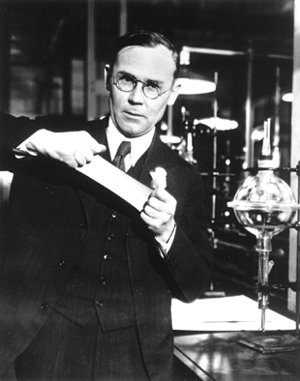
\includegraphics[width=0.24\linewidth]{images/book1/carothers.jpg}

{\small Wallace Carothers en su laboratorio.}
\end{omfigure}

\section{Estructura y propiedades}

Dos muestras del mismo \omterm{def:g12:polymers:polymer}{polímero} pueden comportarse de forma muy distinta:
lo que cuenta es la longitud de las cadenas, su forma y cómo están
empaquetadas.

\begin{proposition}[Cadenas y propiedades]\label{prop:g12:polymers:properties}
\begin{itemize}
  \item Las cadenas más largas se enredan más: el material es más
        resistente y funde a una temperatura más alta.
  \item Las cadenas lineales pueden alinearse unas junto a otras en
        regiones ordenadas, \emph{cristalinas}; las cadenas ramificadas no
        pueden, y quedan desordenadas, \emph{amorfas}. Las regiones
        cristalinas hacen un \omterm{def:g12:polymers:polymer}{polímero} más denso, más rígido y menos
        transparente.
  \item Las cadenas unidas lado a lado solo por fuerzas intermoleculares
        se deslizan unas sobre otras al calentarlas: el \omterm{def:g12:polymers:polymer}{polímero} es un
        \omterm{def:g8:plastics:thermoplastic}{termoplástico}. Las cadenas unidas por \emph{entrecruzamientos}
        covalentes no pueden: el \omterm{def:g12:polymers:polymer}{polímero} es un \omterm{def:g8:plastics:thermoplastic}{termoestable} o, con pocos
        entrecruzamientos, un sólido elástico de tipo caucho.
\end{itemize}
\end{proposition}

\begin{proof}
Calentar da a las cadenas energía suficiente para vencer las fuerzas
intermoleculares que hay entre ellas
(\cref{ch:g11:polarity-and-cohesion}), más débiles que los \omterm{def:g10:lewis-and-shape:covalent-bond}{enlaces
covalentes}; cuanto más contacto hay entre cadenas, más energía hace
falta. Los entrecruzamientos son covalentes: romperlos destruye el
material en lugar de fundirlo.
\end{proof}

\begin{omfigure}
\begin{tikzpicture}[font=\footnotesize, line width=1pt, line cap=round,
    lab/.style={below, align=center, text width=2.8cm}]
  % linear, packed (crystalline)
  \begin{scope}
    \foreach \y in {0,0.25,0.5,0.75,1.0}
      \draw[omDef] plot[smooth, domain=0:2.2, samples=25] (\x, {\y + 0.05*sin(400*\x)});
    \node[lab] at (1.1,-0.2) {cadenas lineales\\ alineadas: cristalino};
  \end{scope}
  % linear, tangled (amorphous)
  \begin{scope}[xshift=3.4cm]
    \draw[omDef] plot[smooth] coordinates {(0,0.2) (0.5,0.9) (1.0,0.3) (1.4,1.1) (2.0,0.5) (2.2,0.9)};
    \draw[omProp] plot[smooth] coordinates {(0,0.9) (0.4,0.3) (0.9,1.0) (1.5,0.2) (1.9,1.0) (2.2,0.3)};
    \draw[black!60] plot[smooth] coordinates {(0.1,0.55) (0.7,0.1) (1.2,0.75) (1.7,0.55) (2.2,0.1)};
    \node[lab] at (1.1,-0.2) {cadenas lineales\\ enredadas: amorfo};
  \end{scope}
  % branched
  \begin{scope}[xshift=6.8cm]
    \draw[omDef] plot[smooth] coordinates {(0,0.5) (0.6,0.6) (1.2,0.45) (1.8,0.65) (2.2,0.5)};
    \draw[omDef] (0.5,0.6) -- (0.35,1.05) (1.0,0.5) -- (1.15,0.05) (1.6,0.6) -- (1.5,1.1) (1.6,0.6) -- (1.95,1.0);
    \node[lab] at (1.1,-0.2) {cadenas\\ ramificadas:\\ no se empaquetan};
  \end{scope}
  % cross-linked
  \begin{scope}[xshift=10.2cm]
    \foreach \y in {0.1,0.55,1.0}
      \draw[omDef] plot[smooth, domain=0:2.2, samples=25] (\x, {\y + 0.06*sin(300*\x)});
    \foreach \x/\a/\b in {0.4/0.1/0.55, 1.3/0.1/0.55, 0.9/0.55/1.0, 1.9/0.55/1.0}
      \draw[omProp, line width=1.6pt] (\x,\a) -- (\x,\b);
    \node[lab] at (1.1,-0.2) {cadenas\\ entrecruzadas:\\ no funden};
  \end{scope}
\end{tikzpicture}

{\small Cuatro disposiciones de cadenas de \omterm{def:g12:polymers:polymer}{polímero}. Los
entrecruzamientos (en naranja) son \omterm{def:g10:lewis-and-shape:covalent-bond}{enlaces covalentes} entre cadenas.}
\end{omfigure}

\begin{example}[Dos polietilenos]\label{ex:g12:polymers:two-pe}
El polietileno fabricado a muy alta presión tiene muchas ramificaciones
cortas: sus cadenas se empaquetan mal, y da películas blandas y
transparentes para bolsas. Fabricado con un \omterm{def:g12:catalysis:catalyst}{catalizador} a baja presión,
sus cadenas son casi lineales y se empaquetan en regiones cristalinas: es
más denso y más rígido, y da botellas de leche y cajas. El mismo
\omterm{def:g12:polymers:polymer}{monómero}, la misma \omterm{def:g12:polymers:repeat-unit}{unidad de repetición}, distinta arquitectura.
\end{example}

\section{Polímeros naturales}

Los seres vivos fabricaron \omterm{def:g12:polymers:polymer}{polímeros} mucho antes que los químicos.

\begin{itemize}
  \item La \textbf{celulosa} y el \textbf{almidón} son cadenas de unidades
        de glucosa, \ce{C6H10O5} por unidad, unidas de forma distinta: la
        celulosa forma fibras rectas y resistentes (madera, algodón,
        papel); el almidón forma espirales que el cuerpo digiere.
  \item Las \textbf{proteínas} son cadenas de aminoácidos unidos por
        enlaces \omterm{def:g11:functional-groups:amine}{amida}, los enlaces peptídicos del dipéptido del
        \cref{ch:g12:synthesis-strategy}.
  \item El \textbf{ADN} es una cadena de nucleótidos; el orden de sus
        cuatro tipos de unidad almacena la información genética.
  \item El \textbf{caucho natural} es un \omterm{def:g12:polymers:addition-polymer}{polímero de adición} del isopreno,
        \ce{CH2=C(CH3)-CH=CH2}, que se recoge como un líquido lechoso, el
        látex, de la corteza del árbol del caucho. Calentado con azufre,
        sus cadenas quedan unidas por puentes de azufre: el caucho se
        vuelve más duro y conserva su forma, como en un neumático.
\end{itemize}

\begin{omfigure}
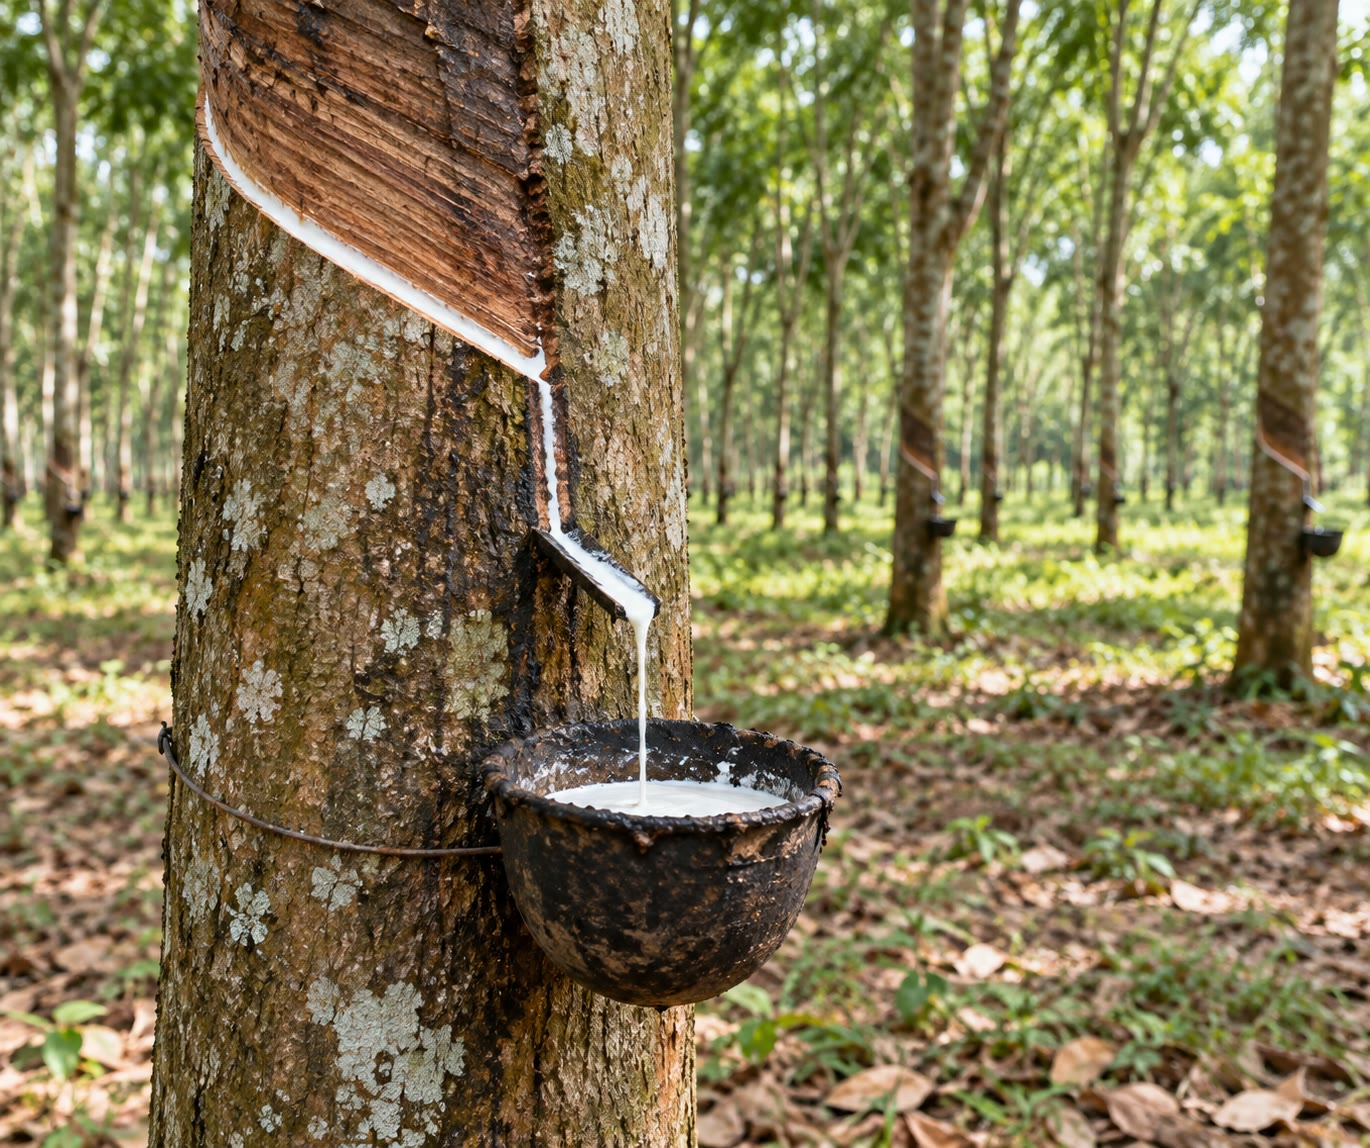
\includegraphics[width=0.45\linewidth]{images/book1/ai/g12-rubber-tapping.jpg}

{\small Sangrado de un árbol del caucho: el látex fluye de un corte en la
corteza a una taza.}
\end{omfigure}

\begin{remark}[Hacer y deshacer]\label{rem:g12:polymers:recycling}
Un \omterm{def:g8:plastics:thermoplastic}{termoplástico} puede fundirse y moldearse de nuevo: es el \omterm{def:g5:raw-materials-and-recycling:recycling}{reciclado}
mecánico. Un \omterm{def:g12:polymers:addition-polymer}{polímero de condensación} también puede descomponerse en sus
\omterm{def:g12:polymers:polymer}{monómeros} mediante la reacción inversa, una hidrólisis, y los \omterm{def:g12:polymers:polymer}{monómeros}
pueden convertirse en \omterm{def:g12:polymers:polymer}{polímero} nuevo: es el \omterm{def:g5:raw-materials-and-recycling:recycling}{reciclado} químico. Un
\omterm{def:g8:plastics:thermoplastic}{termoestable} no admite fácilmente ninguno de los dos.
\end{remark}

\section{Ejercicios}

\begin{exercise}[$\star$]\label{exo:g12:polymers:1}
Da el \omterm{def:g12:polymers:polymer}{monómero} del polipropileno, cuya \omterm{def:g12:polymers:repeat-unit}{unidad de repetición} es
\ce{-CH2-CH(CH3)-}.
\end{exercise}

\begin{exercise}[$\star$]\label{exo:g12:polymers:2}
Escribe la \omterm{def:g12:polymers:repeat-unit}{unidad de repetición} del \omterm{def:g12:polymers:polymer}{polímero} fabricado a partir del
tetrafluoroeteno, \ce{CF2=CF2}. ¿Es un \omterm{def:g12:polymers:addition-polymer}{polímero de adición} o de
condensación?
\end{exercise}

\begin{exercise}[$\star$]\label{exo:g12:polymers:3}
Clasifica como \omterm{def:g12:polymers:addition-polymer}{polímeros de adición} o de condensación: polietileno, PET,
nailon, PVC, poliestireno.
\end{exercise}

\begin{exercise}[$\star$]\label{exo:g12:polymers:4}
¿Cuáles de estos \omterm{def:g12:polymers:polymer}{polímeros} son naturales: celulosa, nailon, almidón, PVC,
caucho del látex, proteínas?
\end{exercise}

\begin{exercise}[$\star$]\label{exo:g12:polymers:5}
¿Por qué cada \omterm{def:g12:polymers:polymer}{monómero} de un \omterm{def:g12:polymers:addition-polymer}{polímero de condensación} debe llevar dos
grupos reactivos?
\end{exercise}

\begin{exercise}[$\star\star$]\label{exo:g12:polymers:6}
Una muestra de PVC tiene una \omterm{def:g10:the-mole:molar-mass}{masa molar} media de \qty{125000}{g/mol}.
Calcula su \omterm{def:g12:polymers:repeat-unit}{grado de polimerización}.
\end{exercise}

\begin{exercise}[$\star\star$]\label{exo:g12:polymers:7}
Una cadena de poliestireno tiene un \omterm{def:g12:polymers:repeat-unit}{grado de polimerización} de 2500.
Calcula su \omterm{def:g10:the-mole:molar-mass}{masa molar}.
\end{exercise}

\begin{exercise}[$\star\star$]\label{exo:g12:polymers:8}
El ácido láctico, \ce{CH3-CH(OH)-COOH}, lleva un grupo \omterm{def:g11:functional-groups:alcohol}{alcohol} y un grupo
ácido. Demuestra que puede formar por sí solo un poliéster, escribe su
\omterm{def:g12:polymers:repeat-unit}{unidad de repetición} y nombra la \omterm{def:g7:atoms-and-molecules:molecule}{molécula} pequeña liberada.
\end{exercise}

\begin{exercise}[$\star\star$]\label{exo:g12:polymers:9}
Explica, con la figura de las disposiciones de las cadenas, por qué las
películas de las bolsas son blandas y transparentes, mientras que las
botellas de leche son rígidas y opacas.
\end{exercise}

\begin{exercise}[$\star\star$]\label{exo:g12:polymers:10}
El mango de una sartén es un \omterm{def:g8:plastics:thermoplastic}{termoestable}, y el pomo de \omterm{def:g8:plastics:plastic}{plástico} de su
tapa también. Describe sus cadenas. ¿Por qué no pueden fundirse y
reciclarse?
\end{exercise}

\begin{exercise}[$\star\star$]\label{exo:g12:polymers:11}
Una cadena de nailon 6,6 tiene una \omterm{def:g10:the-mole:molar-mass}{masa molar} de \qty{22600}{g/mol}.
Calcula la \omterm{def:g10:the-mole:molar-mass}{masa molar} de su \omterm{def:g12:polymers:repeat-unit}{unidad de repetición} \ce{C12H22N2O2}, y
después su \omterm{def:g12:polymers:repeat-unit}{grado de polimerización}.
\end{exercise}

\begin{exercise}[$\star\star\star$]\label{exo:g12:polymers:12}
Escribe la reacción entre una \omterm{def:g7:atoms-and-molecules:molecule}{molécula} de hexano-1,6-diamina y una de
ácido hexanodioico, que da el primer enlace \omterm{def:g11:functional-groups:amine}{amida}. ¿Por qué el producto
puede seguir reaccionando por los dos extremos?
\end{exercise}

\begin{exercise}[$\star\star\star$]\label{exo:g12:polymers:13}
¿Qué masa de agua se libera al fabricar \qty{1.0}{kg} de nailon 6,6?
\end{exercise}

\begin{exercise}[$\star\star\star$]\label{exo:g12:polymers:14}
El caucho natural es blando y pegajoso cuando está caliente; calentado
con azufre, se convierte en el caucho elástico y resistente de los
neumáticos. Explícalo con las cadenas. ¿Por qué es tan difícil reciclar
un neumático?
\end{exercise}

\begin{exercise}[$\star\star\star$]\label{exo:g12:polymers:15}
El almidón y la celulosa tienen la misma fórmula por unidad,
\ce{C6H10O5}. Una cadena de celulosa tiene una \omterm{def:g10:the-mole:molar-mass}{masa molar} de
\qty{1.6e6}{g/mol}. ¿Cuántas unidades de glucosa contiene? ¿Qué longitud
tiene, si cada unidad añade \qty{0.5}{nm} a su longitud?
\end{exercise}

\section{Problema: de la botella al forro polar}

\begin{problem}[{Problema de fin de semana --- ¿cuántas botellas de 25 g hacen falta
para un forro polar?}]
\label{pb:g12:polymers:1}
% ledger: aw:C, aw:H, aw:O
Un forro polar está hecho con \qty{300}{g} de fibra de PET. Se recogen
botellas usadas de \qty{25}{g} cada una, que se clasifican, se lavan, se
trituran, se funden y se hilan; en este proceso, el \qty{80}{\percent} de
la masa de las botellas acaba como fibra en el forro.

\medskip
\noindent\textbf{Parte I --- El \omterm{def:g12:polymers:polymer}{polímero}.}
\begin{enumerate}
  \item Nombra los dos \omterm{def:g12:polymers:polymer}{monómeros} del PET y los \omterm{def:g11:functional-groups:functional-group}{grupos funcionales} que
        llevan.
  \item ¿Qué enlace se forma entre ellos? ¿Qué \omterm{def:g7:atoms-and-molecules:molecule}{molécula} pequeña se
        libera?
  \item ¿Es el PET un \omterm{def:g12:polymers:addition-polymer}{polímero de adición} o de condensación?
  \item Calcula las \omterm{def:g10:the-mole:molar-mass}{masas molares} de los dos \omterm{def:g12:polymers:polymer}{monómeros}.
  \item Deduce la \omterm{def:g10:the-mole:molar-mass}{masa molar} de la \omterm{def:g12:polymers:repeat-unit}{unidad de repetición} \ce{C10H8O4} y
        compruébala con su fórmula.
\end{enumerate}

\medskip
\noindent\textbf{Parte II --- Las cadenas.}
\begin{enumerate}[resume]
  \item El PET de una botella tiene cadenas de \omterm{def:g10:the-mole:molar-mass}{masa molar} media
        \qty{38400}{g/mol}. Calcula el \omterm{def:g12:polymers:repeat-unit}{grado de polimerización}.
  \item ¿Cuántos enlaces \omterm{def:g11:functional-groups:carboxylic-acid}{éster} contiene, aproximadamente, una cadena?
  \item El PET de las botellas es en parte cristalino. ¿Qué dice eso de
        sus cadenas?
  \item ¿Por qué se puede fundir el PET e hilarlo en forma de fibra?
\end{enumerate}

\medskip
\noindent\textbf{Parte III --- El \omterm{def:g5:raw-materials-and-recycling:recycling}{reciclado}.}
\begin{enumerate}[resume]
  \item ¿Qué masa de botellas hace falta para un forro polar?
  \item ¿Cuántas botellas son?
  \item ¿Qué ocurre con el resto de la masa?
  \item ¿Qué principio de la \omterm{def:g12:synthesis-strategy:green-chemistry}{química verde} aplica este \omterm{def:g5:raw-materials-and-recycling:recycling}{reciclado}?
\end{enumerate}

\medskip
\noindent\textbf{Parte IV --- Vuelta a los \omterm{def:g12:polymers:polymer}{monómeros}.}
\begin{enumerate}[resume]
  \item Escribe, para una \omterm{def:g12:polymers:repeat-unit}{unidad de repetición}, la hidrólisis del PET en
        sus \omterm{def:g12:polymers:polymer}{monómeros}.
  \item ¿Qué cantidad de \omterm{def:g12:polymers:repeat-unit}{unidades de repetición} hay en \qty{1.00}{kg} de
        PET?
  \item ¿Qué masas de cada \omterm{def:g12:polymers:polymer}{monómero} da la hidrólisis completa de
        \qty{1.00}{kg} de PET?
  \item ¿Qué masa de agua consume? Comprueba la \omterm{def:g8:balanced-equations:conservation}{conservación de la masa}.
  \item Da una ventaja de este \omterm{def:g5:raw-materials-and-recycling:recycling}{reciclado} químico frente a la fusión.
  \item Da la respuesta final: ¿cuántas botellas de \qty{25}{g} hacen
        falta para un forro polar?
\end{enumerate}
\end{problem}
